\section{Experimental Background}
\subsection{The optical centrifuge}

\begin{frame}{Animation of an accelerating optical centrifuge}
  \centering
  \begin{figure}
  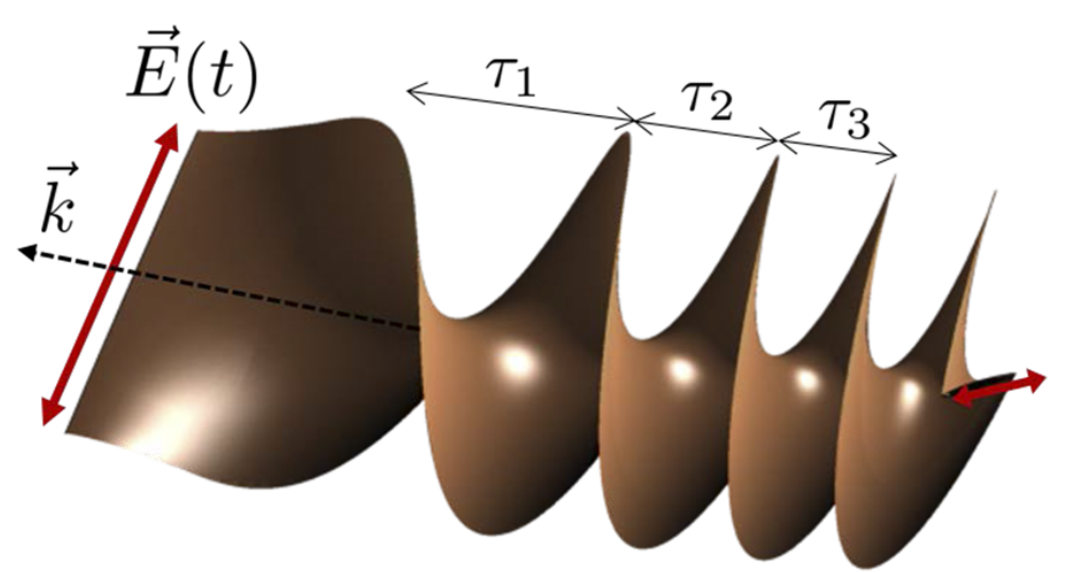
\includegraphics[width=.7\linewidth]{pic/cfg.png}
  \caption{E-field of an accelerating optical centrifuge \footcite{MacPhail_Bartley_2020}}
  \end{figure}
\end{frame}

\begin{frame}{How to make an optical centrifuge}
\small
\begin{minipage}[c]{0.32\textwidth}
  \centering
  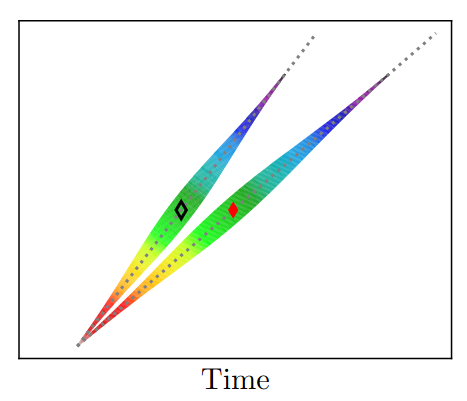
\includegraphics[width=\linewidth]{pic/chirps.png}
  \captionof{figure}{Chirped pulses used to create the accelerating rotating electric field \footcite{wang2025ultraslowopticalcentrifugearbitrarily}}
\end{minipage}\hfill
\begin{minipage}[c]{0.64\textwidth}
  \small
  \begin{itemize}
    \item Take two pulses with \textbf{equal amplitudes} and \textbf{opposite circular polarizations}:
          one right-circular (RCP), one left-circular (LCP).
    \item At any instant, \textbf{RCP + LCP of equal strength} adds up to a \textbf{linearly polarized} electric field.
    \item The \textbf{only thing that matters} for the \emph{direction} of that linear polarization is the
          \textbf{relative optical phase} between the two components.
    \item If that relative phase changes in time, the resulting linear polarization axis \textbf{rotates in time}.
  \end{itemize}
\end{minipage}

\end{frame}
